\section{Python tests}\label{chap-py-test}
We also implemented 6 tests in Python using data coming from different distributions and mixtures to assess the predicting power of the library.
All of them were run with the following settings:
\begin{itemize}
	\item \verb|Neal2| algorithm with 500 iterations, of which 100 for the burn-in phase
	\item Dirichlet process mixture with total mass $m=1$
	\item NNIG hierarchy for the univariate tests and the NNW hierarchy for the multivariate ones
	\item Hyperparameters for all NNIG hierarchies: $\mu_0 = 0.0$, $\lambda = 0.1$, $\alpha = 2$, $\beta = 2$
	\item Hyperparameters for all $d$-dimensional NNW hierarchies: $\mu_0$ is the sample mean of the data, $\lambda = 0.2$, $\nu = d + 3$, $\tau_0 = \frac{1}{\nu} I_d$ (multiple of identity matrix).
\end{itemize}
Data were iid generated through the use of an R script.
Below are listed the first 4 univariate tests alongside their respective sample size and the process from which the data was produced:
\begin{center}
	\begin{tabular}{r|r|l}
		test & $n$ & process \\ \hline
		1 &  200 & $y \sim 0.5 \, \Nc(-3, 1) + 0.5 \, \Nc(3, 1)$ \\
		2 & 1000 & $y \sim 0.9 \, \Nc(-5, 1) + 0.1 \, \Nc(5, 1)$ \\
		3 &  200 & $y \sim 0.3 \, \Nc(-2, 0.8^2) + 0.3 \, \Nc(0, 0.8^2) + 0.4 \, \Nc(2, 1)$ \\
		4 &  400 & $y \sim 0.5 \, t_5(-5, 1 ) + 0.5 \, \text{SkewNormal}(5, 1, 2)$
	\end{tabular}
\end{center}
Test number 4 uses a mixture of the Student's $t$ distribution (refer to \ref{nnig} for more information) and the skew normal distribution (location $\mu=5$, scale $\sigma^2=1$, shape $\alpha=2$). \footnote{Its p.d.f. is as follows ($\phi(t) = (2\pi)^{-1/2} \exp\{-t^2/2\}$ is the standard $\Nc(0,1)$ p.d.f.):
$$
f(x) = 2 \phi\left(\frac{x-\mu}{\sigma^2}\right) \int_{-\infty}^{\alpha \frac{x-\mu}{\sigma^2}} \phi(t) \de t
$$}
Both distributions have similar shapes compared to a Gaussian p.d.f.; in particular, the Student's $t$ converges to the Gaussian one as the degrees of freedom increase, while the skew normal is a generalization which is slightly shifted and tilted on one side, based on the shape parameter (for $\alpha>0$, the distribution moves to the right and is tilted towards the left). \\
Tests 5 and 6 use multivariate data of increasing dimension, $d = 2$ and $d=5$ respectively; for both of them, the sample size is $n=400$ and data is generated from
$$y \sim 0.5 \, \Nc(-3 \cdot 1_d, I_d) + 0.5 \, \Nc(3 \cdot 1_d, I_d)$$
where $1_d$ is the $d$-dimensional unit vector and $I_d$ the $d$-dimensional identity matrix. \\
For each univariate test, a plot was produced that includes the following:
\begin{itemize}
	\item the ``expected prior likelihood'' for the data, i.e. the Gaussian likelihood $\Nc(\mu,\sigma^2)$ with $\mu$ and $\sigma^2$ equal to the expected values provided by their own prior distribution;
	\item the histogram produced by the actual data points used for the test;
	\item the true likelihood from which the data were extracted, as listed in the above table;
	\item the posterior likelihood computed by the library.
\end{itemize}
Having the ``expected prior likelihood'' as a rough starting point, the goal is to approximate the true likelihood via the posterior likelihood by using the given data.
For multivariate tests, we show the following plots, obviously only for the $d=2$ case: posterior likelihood, both in graph and in contour form, and the data histogram. \\
Finally, the adjusted Rand index $ARI$ for the predicted clustering with respect to the true clustering introduced in chapter \ref{chap-py-int} is also listed for all tests.
The results are listed below. \\
The only test the library struggles with is number 3, in which only 2 clusters are recognized instead of the actual 3.
This is due to the fact that the 3 clusters are really close to each other, therefore data for the central one can easily be mistaken as being part of the leftmost and rightmost ones.
\begin{figure}[h]
	\centering
	\begin{minipage}{0.5\textwidth}
		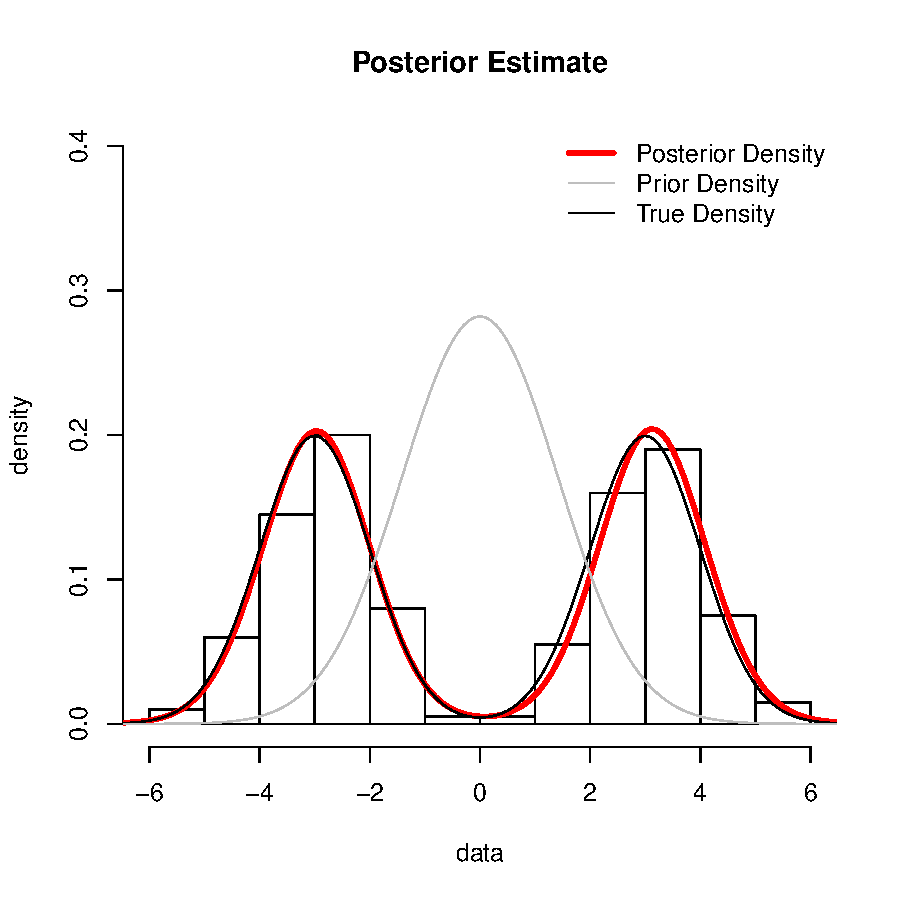
\includegraphics[scale=0.45]{etc/test1.pdf}
		\captionsetup{labelformat=empty}
		\caption{Test 1. $ARI = 1.0$}
	\end{minipage}%
	\begin{minipage}{0.5\textwidth}
		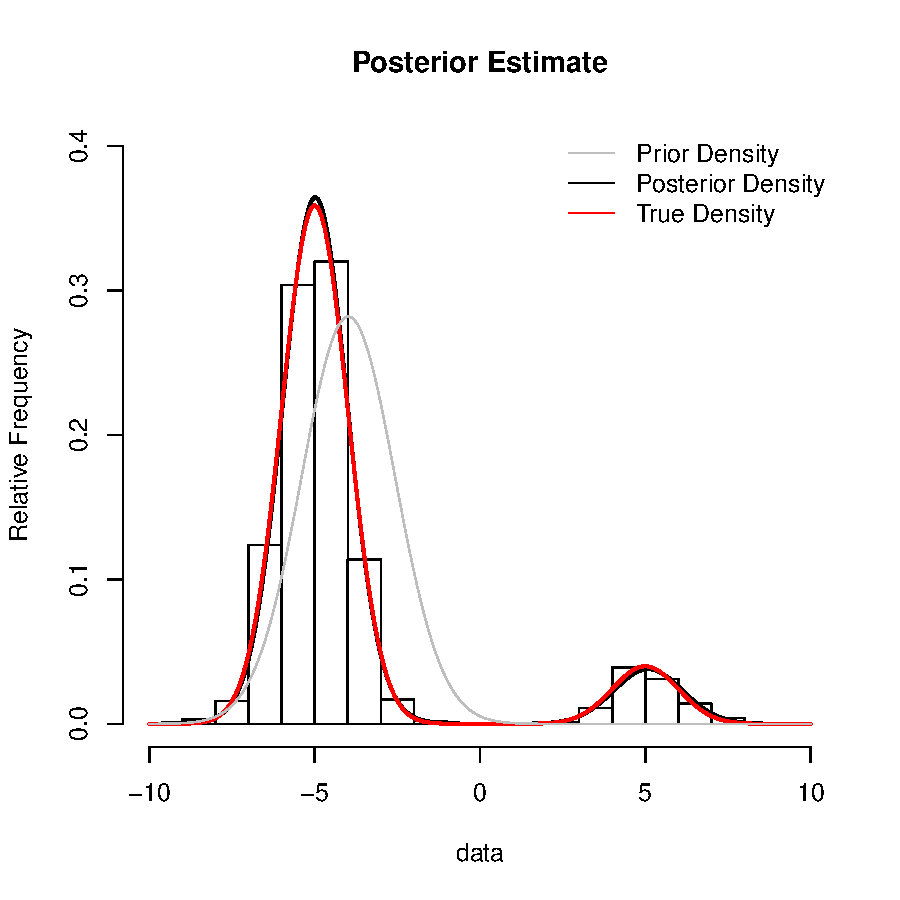
\includegraphics[scale=0.45]{etc/test2.pdf}
		\captionsetup{labelformat=empty}
		\caption{Test 2. $ARI = 1.0$}
	\end{minipage}
\end{figure}

\begin{figure}[h]
	\centering
	\begin{minipage}{0.5\textwidth}
		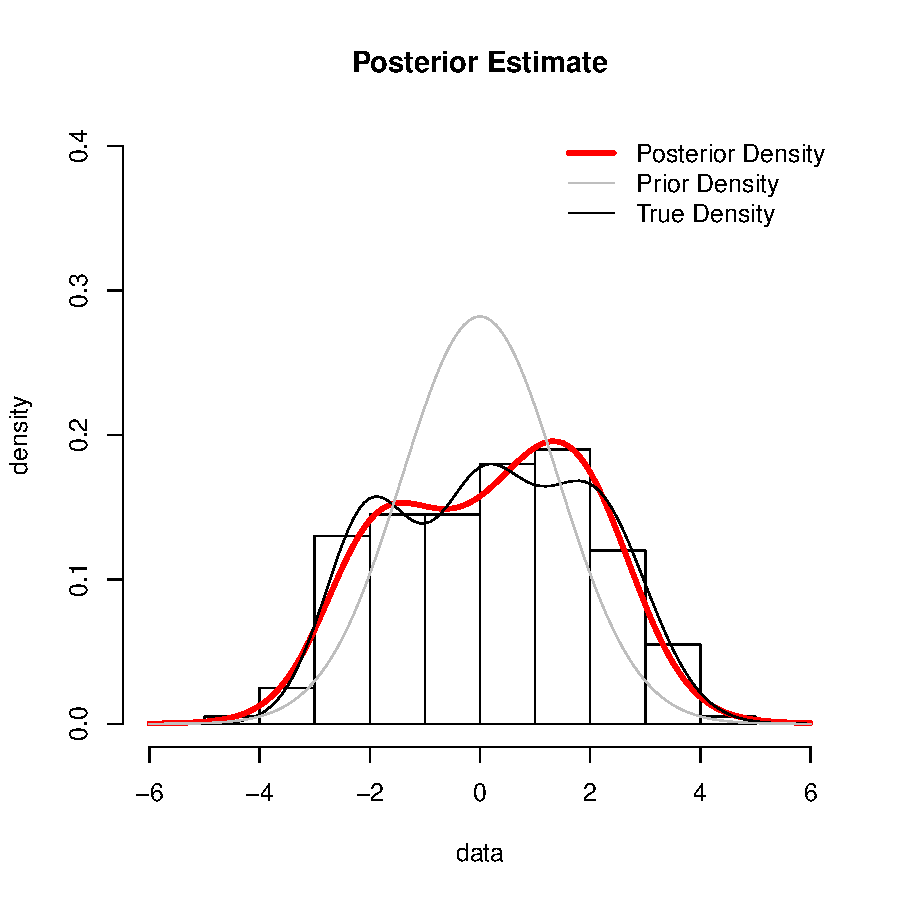
\includegraphics[scale=0.45]{etc/test3.pdf}
		\captionsetup{labelformat=empty}
		\caption{Test 3. $ARI = 0.45$}
	\end{minipage}%
	\begin{minipage}{0.5\textwidth}
		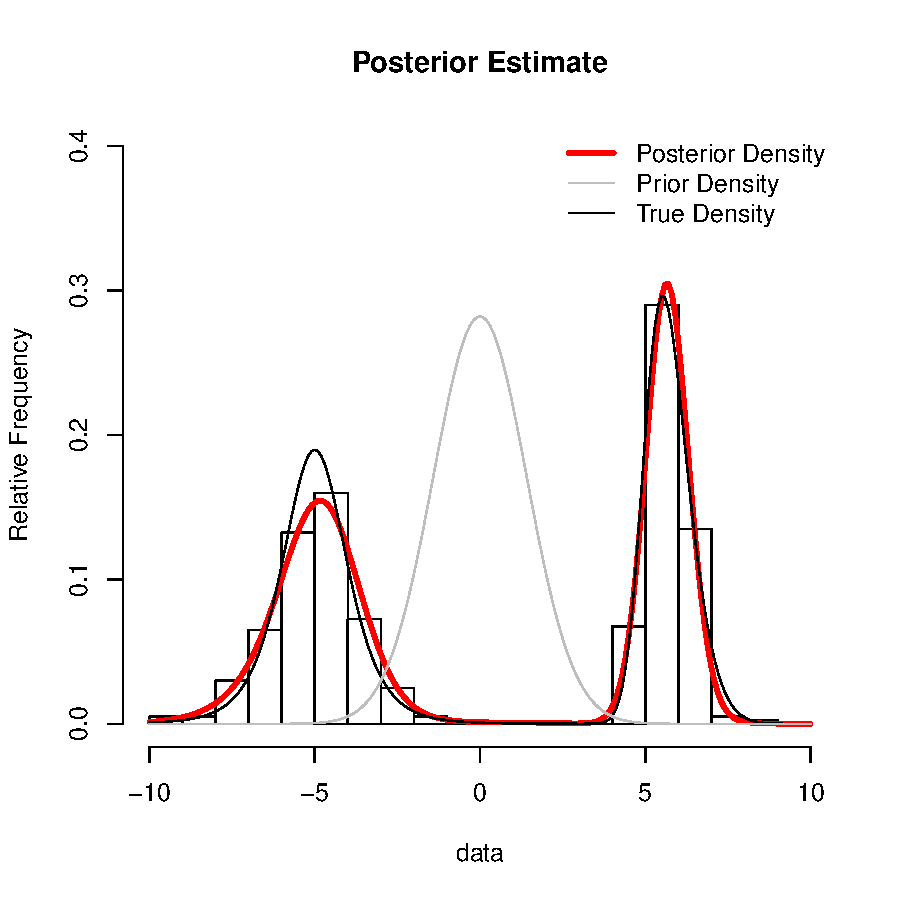
\includegraphics[scale=0.45]{etc/test4.pdf}
		\captionsetup{labelformat=empty}
		\caption{Test 4. $ARI = 0.99$}
	\end{minipage}
\end{figure}

\begin{figure}[h]
	\centering
	\begin{minipage}{0.5\textwidth}
		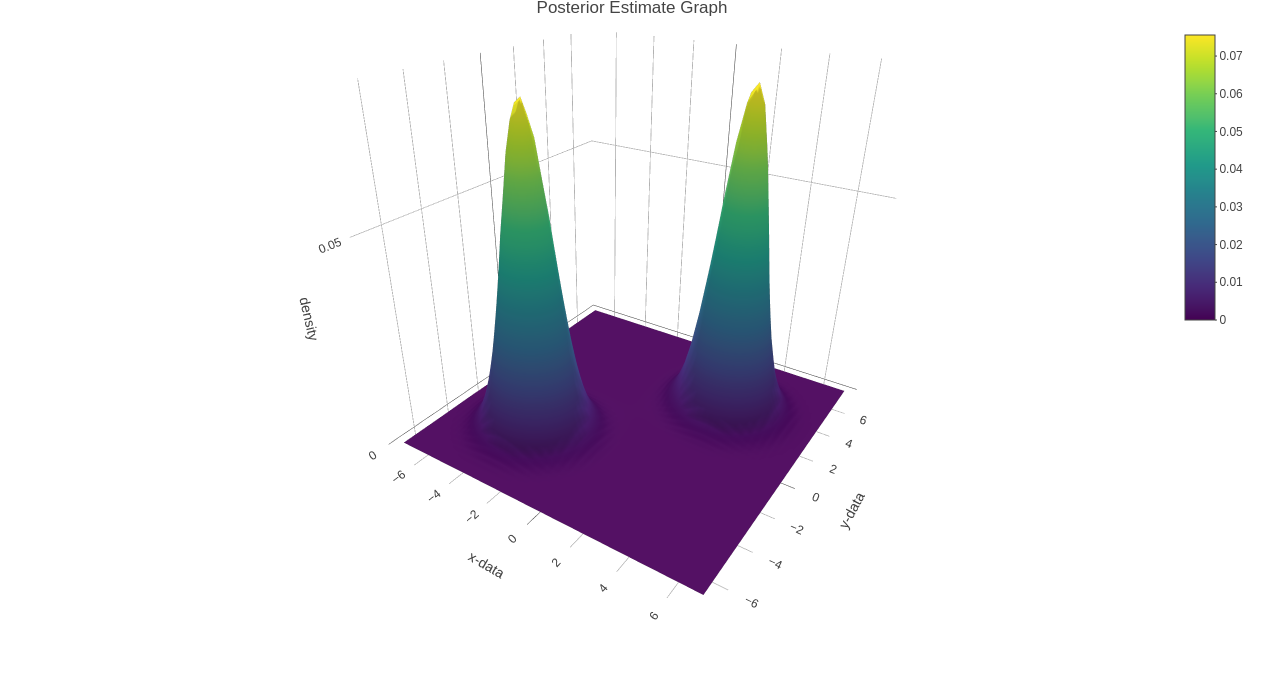
\includegraphics[scale=0.5]{etc/test5_dens.png}
	\end{minipage}%
	\begin{minipage}{0.5\textwidth}
		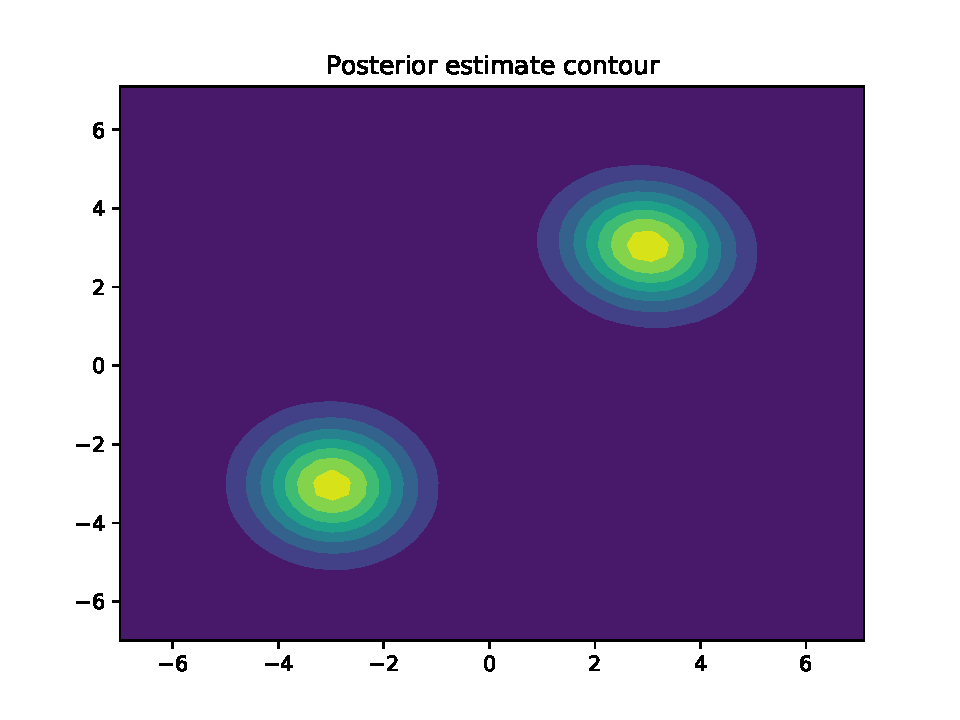
\includegraphics[scale=0.5]{etc/test5_cont.pdf}
	\end{minipage}
	\captionsetup{labelformat=empty}
	\caption{Test 5. $ARI = 1.0$}
\end{figure}


